\documentclass[11pt,a4paper]{article}

\usepackage[T1]{fontenc}
\usepackage[utf8]{inputenc}
\usepackage{lmodern}
\usepackage[english]{babel}
\usepackage[margin=2.3cm]{geometry}
\usepackage{graphicx}
\usepackage{booktabs}
\usepackage{array}
\usepackage{longtable}
\usepackage{multirow}
\usepackage{amsmath}
\usepackage{amssymb}
\usepackage{xcolor}
\usepackage{caption}
\usepackage{subcaption}
\usepackage{float}
\usepackage{enumitem}
\usepackage{fancyhdr}
\usepackage[hidelinks]{hyperref}

\definecolor{primary}{HTML}{1F3B6E}
\definecolor{accent}{HTML}{E26D3C}
\definecolor{green}{HTML}{2E7D5B}
\definecolor{red}{HTML}{C04432}
\definecolor{panel}{HTML}{F1F4F9}

\captionsetup{font=small,labelfont={bf,color=primary}}
\graphicspath{{../results/figures/}{../results/confusion_matrices/}}
\setlength{\parskip}{0.5em}
\setlength{\parindent}{0pt}
\renewcommand{\arraystretch}{1.2}

\pagestyle{fancy}
\fancyhf{}
\fancyhead[L]{\small\textcolor{primary}{Predicting User Sentiment in Software Issue Reports}}
\fancyhead[R]{\small\textcolor{primary}{ST2MLE}}
\fancyfoot[C]{\small\thepage}
\renewcommand{\headrulewidth}{0.4pt}

\newcommand{\sectionrule}{\textcolor{accent}{\rule{\linewidth}{1.2pt}}}

\begin{document}

% ============================== TITLE PAGE ==============================
\begin{titlepage}
\centering
\vspace*{1.8cm}
{\color{primary}\Huge\bfseries Predicting User Sentiment\\[0.3cm] in Software Issue Reports\par}
\vspace{0.6cm}
\sectionrule\par
\vspace{0.6cm}
{\Large A complete, reproducible machine learning pipeline for the\\
three-class sentiment classification of application reviews\par}
\vspace{2.0cm}
{\large\bfseries Yann MASSOUAMA \quad$\cdot$\quad Vénus BAKIKO \quad$\cdot$\quad Faïçal DIELO\par}
\vspace{0.8cm}
{\large ST2MLE --- Machine Learning for IT Engineers\par}
\vspace{0.3cm}
{\large Technical project report\par}
\vfill
{\small All tables, figures and numerical values reported in this document are
produced programmatically by \texttt{python main.py} and are fully reproducible:
a single global seed (\texttt{RANDOM\_STATE = 42}) is threaded through data
splitting, cross-validation shuffling and every stochastic estimator.\par}
\vspace{0.5cm}
{\small\today\par}
\end{titlepage}

\tableofcontents
\newpage

% ============================== ABSTRACT ==============================
\section*{Abstract}
\addcontentsline{toc}{section}{Abstract}
This report presents the design, implementation and evaluation of a complete
supervised machine learning pipeline for classifying the sentiment of user-written
application reviews into three classes: \emph{negative}, \emph{neutral} and
\emph{positive}. Working from a real, pre-cleaned corpus of Facebook application
reviews, we compare four text-vectorisation strategies (Bag of Words, TF-IDF, an
in-domain Word2Vec model and the pre-trained Google News Word2Vec vectors) against
five classifiers (Naive Bayes, Decision Tree, Random Forest, AdaBoost and Logistic
Regression), for a total of twenty tuned vectoriser--classifier combinations. Each
classifier is optimised by grid search under five-fold stratified cross-validation,
using the macro-averaged F1 score as the selection criterion because the corpus is
strongly imbalanced. Four further experiments study, respectively, class-imbalance
handling (SMOTE versus random under-sampling), dimensionality reduction (Truncated
SVD), decision-tree pruning (cost-complexity pruning) and early stopping in gradient
boosting. The best configuration, TF-IDF with multinomial Naive Bayes, attains a
macro-F1 of $0.559$ on the held-out test set. Beyond the raw numbers, the study makes
a clear methodological point: on an imbalanced dataset, accuracy is deceptive (a model
can reach $0.84$ accuracy while never predicting the minority class), the macro-F1 and
the per-class recall expose this failure, and resampling is what allows the minority
class to appear in the predictions, at a measurable cost in majority accuracy.

% ============================== 1. INTRODUCTION ==============================
\section{Introduction}
Software is now delivered to millions of users who continuously express opinions about
it: through application-store reviews, bug reports, feature requests and issue-tracker
comments. This feedback is a strategic asset. It tells development teams what users
love, what frustrates them, and which defects hurt the product most. The difficulty is
one of scale: a popular application receives thousands of reviews per day, far more
than any team can read manually. \emph{Sentiment analysis}, the automatic detection of
the emotional polarity of a piece of text, is the standard answer to this problem. By
labelling each review as negative, neutral or positive, a team can monitor user
satisfaction over time, triage the most urgent complaints, and quantify the effect of a
release.

This project addresses precisely that task. We build, from raw text to evaluated
predictions, a machine learning pipeline that reads the body of an application review
and assigns it one of three sentiment classes. The work is deliberately framed as a
\emph{comparative study} rather than the pursuit of a single model: the brief for the
\emph{ST2MLE --- Machine Learning for IT Engineers} course asks not only for a working
classifier but for an explicit comparison of several ways of representing text and
several classification algorithms, together with cross-validation, hyper-parameter
tuning, class-imbalance handling, dimensionality reduction, tree pruning, regularisation
and early stopping. Each of these requirements is implemented, measured and discussed.

\subsection{Objectives}
The objectives of the project are the following.
\begin{enumerate}[leftmargin=1.6em,itemsep=1pt]
\item Assemble a reproducible, end-to-end pipeline from raw review text to a final,
honestly measured sentiment prediction.
\item Compare four vectorisation strategies and five classifiers under a single,
rigorous evaluation protocol, and identify the best combination with evidence.
\item Study, in dedicated experiments, the techniques that the course requires:
class-imbalance correction, dimensionality reduction, pruning, regularisation and
early stopping.
\item Select and justify metrics that are meaningful on an imbalanced problem, and use
them to interpret every result, including the failure modes of the models.
\end{enumerate}

\subsection{Structure of this report}
Section~\ref{sec:problem} reviews the problem and the relevant background. Section~%
\ref{sec:data} describes the dataset and its preparation. Section~\ref{sec:method}
details the full methodology, from preprocessing to the evaluation protocol. Section~%
\ref{sec:metrics} explains the performance metrics and their meaning in our context.
Section~\ref{sec:results} presents the main comparison of all twenty combinations.
Section~\ref{sec:matrices} reproduces and comments on every confusion matrix
individually. Sections~\ref{sec:imbalance} to~\ref{sec:earlystopping} cover the four
focused experiments. Section~\ref{sec:discussion} discusses the findings and
trade-offs, and Section~\ref{sec:conclusion} concludes with perspectives for future
work.

% ============================== 2. PROBLEM ==============================
\section{Problem statement and background}
\label{sec:problem}
\subsection{Formal definition}
Let $\mathcal{D} = \{(d_i, y_i)\}_{i=1}^{N}$ be a corpus of $N$ reviews, where each
$d_i$ is a string of natural-language text and each label
$y_i \in \{\text{negative}, \text{neutral}, \text{positive}\}$. We seek a function
$f : \text{text} \rightarrow \{\text{negative}, \text{neutral}, \text{positive}\}$
that generalises from a training subset to unseen reviews. Because the output space has
three mutually exclusive values, this is a \emph{single-label, multi-class}
classification problem, as opposed to binary sentiment (positive versus negative) or
multi-label tagging. Text cannot be consumed directly by the learning algorithms, so
the pipeline first maps each document to a numerical feature vector
$\phi(d_i) \in \mathbb{R}^m$ through a \emph{vectoriser}, and the classifier then learns
the mapping from $\mathbb{R}^m$ to the label space.

\subsection{Why the task is non-trivial}
Three properties make this problem genuinely difficult and are worth stating early,
because they explain many of the results that follow.
\begin{itemize}[leftmargin=1.4em,itemsep=1pt]
\item \textbf{Proxy labels.} Our ground-truth labels are derived from star ratings, not
from a human annotation of sentiment. A star rating is a convenient but imperfect proxy:
a three-star review (mapped to \emph{neutral}) often reads like a faint complaint or a
lukewarm endorsement, so the neutral class overlaps its neighbours by construction.
\item \textbf{Severe class imbalance.} As in most app stores, positive reviews vastly
outnumber the rest, and the neutral class is tiny. A classifier can therefore obtain a
high accuracy simply by predicting the majority class, which makes accuracy a poor and
even misleading objective.
\item \textbf{Short, informal text.} Reviews are short, contain slang, abbreviations,
emoji and spelling mistakes, and are sometimes written in another language. The
sentiment of a short review often hinges on one or two words, which has direct
consequences for the choice of representation.
\end{itemize}

\subsection{Families of text representation}
Turning text into vectors is the central modelling decision, and the literature offers
two broad families, both of which we evaluate.
\emph{Count-based} representations describe a document by the words it contains. Bag of
Words records raw counts; TF-IDF re-weights those counts so that words which are
frequent in a document but rare across the corpus (and therefore discriminative)
receive more weight. These representations are high-dimensional and sparse, and they
preserve the identity of individual words, which matters when a single keyword carries
the sentiment.
\emph{Embedding-based} representations map each word to a dense, low-dimensional vector
learned so that words used in similar contexts lie close together. Word2Vec is the
canonical example. A document can then be represented by the mean of its word vectors.
Embeddings capture semantic similarity but, when averaged over a document, they tend to
dilute the few strong sentiment words that a short review relies on. This tension
between count-based and embedding-based representations is one of the themes of our
results.

% ============================== 3. DATASET ==============================
\section{Dataset and data preparation}
\label{sec:data}
\subsection{Source and labelling convention}
We use a real, publicly available dataset of Facebook application reviews exported from
Kaggle. Each record contains the review text (the \texttt{content} field) and an integer
star rating from one to five (the \texttt{score} field). We convert the rating into a
sentiment label using the standard convention summarised in Table~\ref{tab:starmap}.
This mapping is deterministic and is the single source of supervision in the project.
As noted above, the star rating is a proxy for sentiment, and the three-star to neutral
mapping is the principal source of label noise.

\begin{table}[H]
\centering
\begin{tabular}{cl}
\toprule
\textbf{Star rating} & \textbf{Assigned sentiment} \\
\midrule
1 or 2 stars & negative \\
3 stars      & neutral \\
4 or 5 stars & positive \\
\bottomrule
\end{tabular}
\caption{Star-to-sentiment mapping used throughout the project.}
\label{tab:starmap}
\end{table}

\subsection{De-duplication and cleaning of empty documents}
Application reviews contain a very large number of duplicate short texts; the strings
``good'', ``nice'' or ``love it'' each appear hundreds of times. We remove duplicate
review texts for a subtle but important reason: if an identical string appeared in both
the training and the test partition, the model would be evaluated on text it has already
seen, and the reported score would be optimistically biased. After de-duplication, and
after dropping the reviews that become empty once cleaning removes all of their content
(emoji-only reviews, or reviews written entirely in a non-English script), $5\,923$
unique reviews remain.

\subsection{Class distribution}
The resulting class distribution, shown in Table~\ref{tab:dist} and
Figure~\ref{fig:dist}, is strongly imbalanced. Positives represent roughly $64\%$ of the
corpus, negatives roughly $31\%$, and the neutral class only about $4.5\%$. Positives
outnumber neutrals by approximately fourteen to one. This imbalance is not an artefact
to be removed; it is a realistic property of app-store feedback, and handling it
correctly is one of the explicit goals of the study.

\begin{table}[H]
\centering
\begin{tabular}{lccc}
\toprule
\textbf{Class} & \textbf{From rating} & \textbf{Count} & \textbf{Share} \\
\midrule
positive & 4 to 5 stars & $3\,801$ & $64.2\%$ \\
negative & 1 to 2 stars & $1\,857$ & $31.4\%$ \\
neutral  & 3 stars      & $265$    & $4.5\%$ \\
\midrule
\textbf{total} & & $\mathbf{5\,923}$ & $100\%$ \\
\bottomrule
\end{tabular}
\caption{Class distribution after cleaning and de-duplication.}
\label{tab:dist}
\end{table}

\begin{figure}[H]
\centering
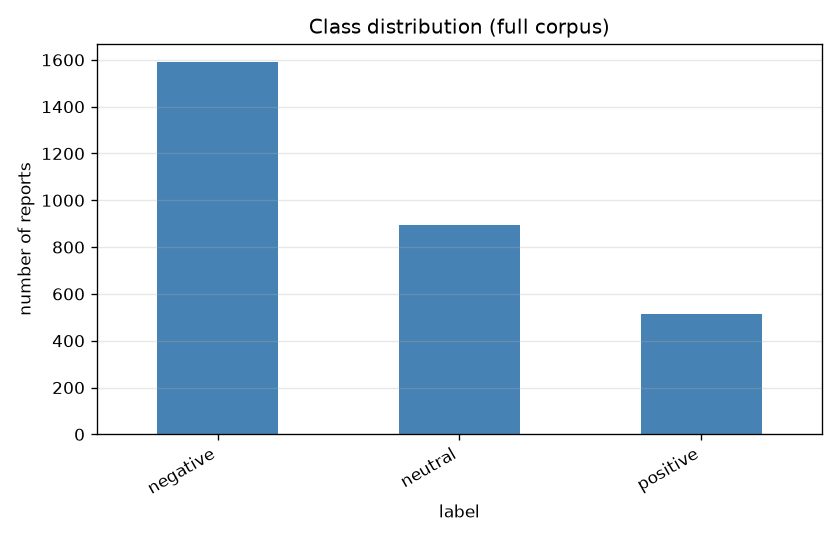
\includegraphics[width=0.6\linewidth]{class_distribution.png}
\caption{Number of reviews per class on the full corpus. The neutral class is tiny,
which drives most of the difficulty analysed later in the report.}
\label{fig:dist}
\end{figure}

\begin{figure}[H]
\centering
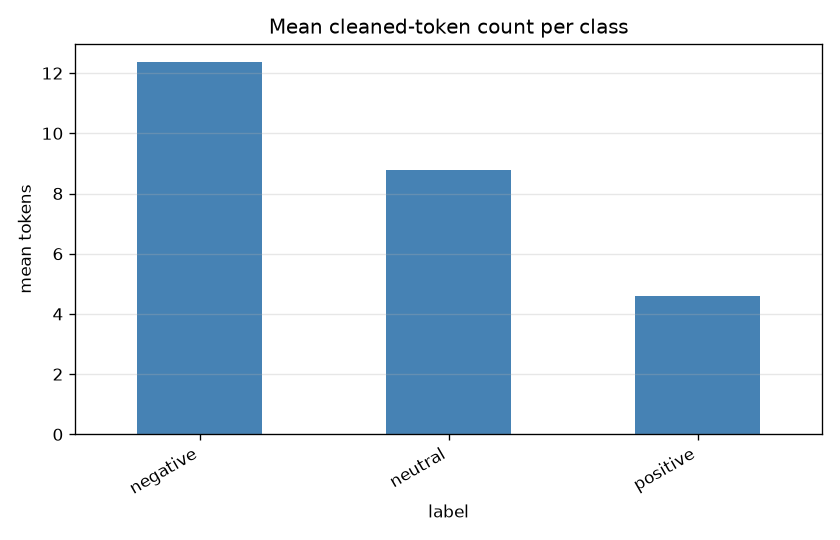
\includegraphics[width=0.6\linewidth]{token_length_by_class.png}
\caption{Mean number of cleaned tokens per class. The three classes have comparable
average lengths, so document length alone is not a discriminative cue and the models
must rely on the words themselves.}
\label{fig:length}
\end{figure}

% ============================== 4. METHODOLOGY ==============================
\section{Methodology}
\label{sec:method}
The pipeline reads, from left to right: raw text $\rightarrow$ preprocessing
$\rightarrow$ vectorisation $\rightarrow$ optional balancing $\rightarrow$ optional
dimensionality reduction $\rightarrow$ a tuned classifier $\rightarrow$ evaluation. Two
engineering decisions keep the whole study both fast and methodologically sound. First,
preprocessing learns nothing from the data (it is \emph{stateless}), so it is applied a
single time up front, which is exactly equivalent to running it inside every
cross-validation fold but avoids re-lemmatising the corpus thousands of times. Second,
the fitted vectorisers are cached on disk with a shared \texttt{joblib.Memory} against a
single fixed cross-validation splitter, so the expensive Word2Vec and TF-IDF fits are
computed once per fold and reused across every hyper-parameter combination and every
classifier. The complete study runs in roughly eight minutes on four cores.

\subsection{Preprocessing}
Each review is normalised through the classical natural-language sequence
\emph{normalise $\rightarrow$ tokenise $\rightarrow$ remove stop-words $\rightarrow$
lemmatise}, with two deliberate, sentiment-aware refinements.
\begin{enumerate}[leftmargin=1.6em,itemsep=2pt]
\item \textbf{Normalisation.} The text is lower-cased; URLs, HTML tags, punctuation and
digits are removed; and runs of whitespace are collapsed. Only alphabetic tokens
survive.
\item \textbf{Tokenisation.} The cleaned string is split into word tokens.
\item \textbf{Stop-word removal with a negation whitelist.} Common, low-information
words (``the'', ``a'', ``is'') are removed, \emph{except} negation cues such as
``not'', ``no'', ``never'', ``without'' and ``cannot''. This exception is important:
the phrases ``working'' and ``not working'' carry opposite sentiment, and discarding
``not'' as an ordinary stop-word would destroy that signal.
\item \textbf{Lemmatisation.} A light two-pass WordNet lemmatisation maps each token
first to its verb lemma and then to its noun lemma, so that ``crashing'' becomes
``crash'' and ``issues'' becomes ``issue''. This shrinks the vocabulary and groups
inflected forms of the same word without the computational cost of a full
part-of-speech tagger.
\end{enumerate}
As a concrete example, the raw review \texttt{"Critical issue, the app keeps
crashing!!!"} is transformed into \texttt{"critical issue app keep crash"}.

\subsection{Vectorisation}
\label{sec:vec}
We compare the four representations named in the brief, summarised in
Table~\ref{tab:vec}. Bag of Words and TF-IDF both produce high-dimensional, sparse and
non-negative vectors; they differ only in the weighting. For TF-IDF we enable
sublinear term-frequency scaling, a minimum document frequency of two (so that terms
appearing in a single document are dropped as noise), a vocabulary capped at the
$5\,000$ most frequent terms, and an n-gram range of $(1,2)$ so that informative word
pairs such as ``not good'' are captured alongside single words. The in-domain Word2Vec
model is trained on our own reviews ($100$-dimensional vectors, context window of five,
thirty epochs); a document is represented by the mean of its word vectors. The
pre-trained variant reuses the publicly available Google News Word2Vec vectors
($300$-dimensional, trained on roughly one hundred billion words), which is the exact
\emph{pre-trained Word2Vec} the brief refers to. Keeping both an in-domain and a
pre-trained embedding lets us contrast learning representations on our own, limited data
against reusing representations learned on a very large external corpus, a form of
transfer learning.

\begin{table}[H]
\centering
\begin{tabular}{lll}
\toprule
\textbf{Method} & \textbf{Underlying idea} & \textbf{Output} \\
\midrule
Bag of Words & raw count of each word & sparse, non-negative \\
TF-IDF & counts re-weighted by inverse document frequency & sparse, non-negative \\
Word2Vec (in-domain) & mean of embeddings trained on our reviews & dense \\
Word2Vec (pre-trained) & mean of Google News $300$d vectors & dense \\
\bottomrule
\end{tabular}
\caption{The four vectorisers. Sparse, non-negative outputs feed multinomial Naive
Bayes; dense outputs use the Gaussian variant, selected automatically.}
\label{tab:vec}
\end{table}

A BERT vectoriser is also implemented and documented in the code base. It requires the
optional deep-learning stack and network access to the model hub, which is not reachable
in our execution environment, so it is skipped automatically and provided through a
dedicated script that runs wherever the hub is available, for example on Google Colab.

\subsection{Classifiers and their hyper-parameters}
\label{sec:clf}
We compare five classifiers, chosen so that together they cover the techniques the
brief requires (pruning, ensembles, boosting and regularisation). For each one, the
hyper-parameters listed in Table~\ref{tab:grids} are tuned by grid search; the values
were chosen to be broad enough to demonstrate meaningful tuning yet compact enough to
remain fast under five-fold cross-validation.

\begin{table}[H]
\centering
\small
\begin{tabular}{lll}
\toprule
\textbf{Classifier} & \textbf{Tuned hyper-parameter} & \textbf{Values searched} \\
\midrule
Naive Bayes (multinomial) & \texttt{alpha} (Laplace smoothing) & $0.1,\ 0.5,\ 1.0$ \\
Naive Bayes (Gaussian) & \texttt{var\_smoothing} & $10^{-9},\ 10^{-8},\ 10^{-7}$ \\
\midrule
\multirow{3}{*}{Decision Tree} & \texttt{max\_depth} (pre-pruning) & None,$\ 10,\ 20,\ 30$ \\
 & \texttt{min\_samples\_leaf} (pre-pruning) & $1,\ 5,\ 10$ \\
 & \texttt{ccp\_alpha} (post-pruning) & $0,\ 10^{-3},\ 10^{-2}$ \\
\midrule
\multirow{4}{*}{Random Forest} & \texttt{n\_estimators} & $200$ \\
 & \texttt{max\_depth} & None,$\ 20$ \\
 & \texttt{min\_samples\_leaf} & $1,\ 2$ \\
 & \texttt{max\_features} & \texttt{sqrt} \\
\midrule
\multirow{2}{*}{AdaBoost} & \texttt{n\_estimators} & $100,\ 200$ \\
 & \texttt{learning\_rate} & $0.5,\ 1.0$ \\
\midrule
Logistic Regression & \texttt{C} (inverse L2 strength) & $0.1,\ 1.0,\ 10.0$ \\
\bottomrule
\end{tabular}
\caption{Hyper-parameter grids per classifier. The Naive Bayes variant is selected
automatically: multinomial for sparse count features, Gaussian for dense embeddings.}
\label{tab:grids}
\end{table}

The intuition behind each model is as follows. \textbf{Naive Bayes} estimates, for each
class, the probability of each word, and predicts the class that maximises the product
of the prior and the word likelihoods; it assumes the words are conditionally
independent, which is false in practice but works very well and is extremely fast in
high dimension. The Laplace smoothing parameter \texttt{alpha} prevents a single unseen
word from forcing a zero probability. \textbf{The Decision Tree} is interpretable but
tends to over-fit, which is exactly why both its pre-pruning parameters
(\texttt{max\_depth}, \texttt{min\_samples\_leaf}) and its post-pruning parameter
(\texttt{ccp\_alpha}) are placed in the grid. \textbf{The Random Forest} averages many
de-correlated trees and is a strong low-variance ensemble. \textbf{AdaBoost} combines
many very shallow trees, re-weighting the hard cases at each round. \textbf{Logistic
Regression} draws a regularised linear boundary; tuning its inverse-strength parameter
\texttt{C} is our explicit demonstration of L2 regularisation, where a small \texttt{C}
regularises strongly (a simpler model, less over-fitting) and a large \texttt{C} lets
the model fit the data more closely.

\subsection{Evaluation protocol}
The data is split into $80\%$ training and $20\%$ test in a stratified manner, so that
the three class proportions are preserved in both partitions. On the training set we run
five-fold stratified cross-validation and tune every classifier with a grid search that
maximises the macro-averaged F1 score. Crucially, the held-out test set is touched only
once, at the very end, to report the final numbers, and any resampling is performed
inside the pipeline so that it acts on the training folds alone and never on the
validation or test data. Every stochastic component is seeded, so a clean run reproduces
the same results exactly. The five-fold cross-validation, illustrated conceptually in
the rotation where each of the five folds serves once as the validation set while the
other four train the model, yields a stable and honest estimate of generalisation
performance and prevents the hyper-parameter choice from over-fitting a single lucky
split.

% ============================== 5. METRICS ==============================
\section{Performance metrics and their meaning}
\label{sec:metrics}
Because the problem has three classes, each metric is defined per class (one class
against the rest) and then averaged. For a given class, a \emph{true positive} is a
review that truly belongs to the class and is predicted as such; a \emph{false
positive} is a review predicted as the class but truly belonging to another; and a
\emph{false negative} is a true member of the class that the model assigned elsewhere.

\begin{itemize}[leftmargin=1.4em,itemsep=2pt]
\item \textbf{Accuracy} is the proportion of correctly classified reviews over the whole
test set. On an imbalanced problem it is misleading, because a model can score high by
always predicting the dominant class.
\item \textbf{Precision} of a class, $\text{TP}/(\text{TP}+\text{FP})$, answers: when the
model predicts this class, how often is it right? It measures the reliability of the
predictions for that class.
\item \textbf{Recall} of a class, $\text{TP}/(\text{TP}+\text{FN})$, answers: among the
reviews that truly belong to this class, how many does the model recover? It measures
coverage.
\item \textbf{F1} is the harmonic mean of precision and recall,
$2\,PR/(P+R)$, so it is low whenever either of the two is low; it cannot be high unless
both are.
\item \textbf{Macro-F1} is the unweighted mean of the three per-class F1 scores. It
treats every class equally regardless of its size, so neglecting the rare class is
penalised heavily.
\end{itemize}

This is precisely why we tune on the macro-F1 rather than on accuracy. On a corpus that
is $64\%$ positive, accuracy rewards a model that ignores the minority classes, whereas
the macro-F1 and the per-class recall expose that behaviour immediately. The
\emph{macro} average (each class counts equally) must be distinguished from the
\emph{micro} average (each review counts equally, which on this corpus is dominated by
the positive class and behaves like accuracy). Throughout the report, the macro-F1 and
the per-class recall are the headline numbers; accuracy is reported for completeness but
is never the basis of a decision.

% ============================== 6. RESULTS ==============================
\section{Results: comparison of all twenty combinations}
\label{sec:results}
Table~\ref{tab:main} reports the test-set results for all twenty vectoriser--classifier
combinations, sorted by macro-F1. The column \textbf{CV F1} is the mean macro-F1 across
the five cross-validation folds on the training set (the criterion used for tuning),
while the remaining columns are computed once on the held-out test set.
Figures~\ref{fig:cmpf1} and~\ref{fig:cmpacc} display the same information graphically.

\begin{table}[H]
\centering
\small
\begin{tabular}{rllccccc}
\toprule
\# & \textbf{Vectoriser} & \textbf{Classifier} & \textbf{CV F1} & \textbf{Acc.} & \textbf{Prec.} & \textbf{Rec.} & \textbf{F1 macro} \\
\midrule
1  & TF-IDF & Naive Bayes & $0.550$ & $0.839$ & $0.550$ & $0.569$ & $\mathbf{0.559}$ \\
2  & TF-IDF & Logistic Regression & $0.557$ & $0.830$ & $0.547$ & $0.563$ & $0.555$ \\
3  & TF-IDF & Random Forest & $0.541$ & $0.824$ & $0.540$ & $0.558$ & $0.548$ \\
4  & BoW & Naive Bayes & $0.569$ & $0.817$ & $0.542$ & $0.554$ & $0.548$ \\
5  & BoW & Logistic Regression & $0.561$ & $0.806$ & $0.550$ & $0.545$ & $0.546$ \\
6  & Word2Vec pre-trained & Random Forest & $0.535$ & $0.821$ & $0.542$ & $0.545$ & $0.542$ \\
7  & BoW & Decision Tree & $0.533$ & $0.768$ & $0.547$ & $0.533$ & $0.539$ \\
8  & BoW & Random Forest & $0.542$ & $0.810$ & $0.534$ & $0.542$ & $0.537$ \\
9  & Word2Vec & Logistic Regression & $0.532$ & $0.810$ & $0.527$ & $0.547$ & $0.537$ \\
10 & Word2Vec pre-trained & Logistic Regression & $0.558$ & $0.802$ & $0.525$ & $0.544$ & $0.535$ \\
11 & Word2Vec & Random Forest & $0.539$ & $0.801$ & $0.520$ & $0.542$ & $0.530$ \\
12 & TF-IDF & Decision Tree & $0.527$ & $0.784$ & $0.578$ & $0.530$ & $0.528$ \\
13 & Word2Vec & Naive Bayes & $0.517$ & $0.685$ & $0.542$ & $0.537$ & $0.518$ \\
14 & Word2Vec & AdaBoost & $0.518$ & $0.780$ & $0.503$ & $0.531$ & $0.516$ \\
15 & Word2Vec pre-trained & AdaBoost & $0.527$ & $0.783$ & $0.506$ & $0.527$ & $0.516$ \\
16 & Word2Vec & Decision Tree & $0.533$ & $0.763$ & $0.496$ & $0.514$ & $0.505$ \\
17 & Word2Vec pre-trained & Decision Tree & $0.506$ & $0.746$ & $0.483$ & $0.504$ & $0.493$ \\
18 & TF-IDF & AdaBoost & $0.459$ & $0.757$ & $0.512$ & $0.471$ & $0.472$ \\
19 & BoW & AdaBoost & $0.454$ & $0.753$ & $0.516$ & $0.463$ & $0.465$ \\
20 & Word2Vec pre-trained & Naive Bayes & $0.444$ & $0.630$ & $0.465$ & $0.479$ & $0.455$ \\
\bottomrule
\end{tabular}
\caption{Full comparison on the held-out test set, sorted by macro-F1. The best
configuration is TF-IDF with Naive Bayes.}
\label{tab:main}
\end{table}

\begin{figure}[H]
\centering
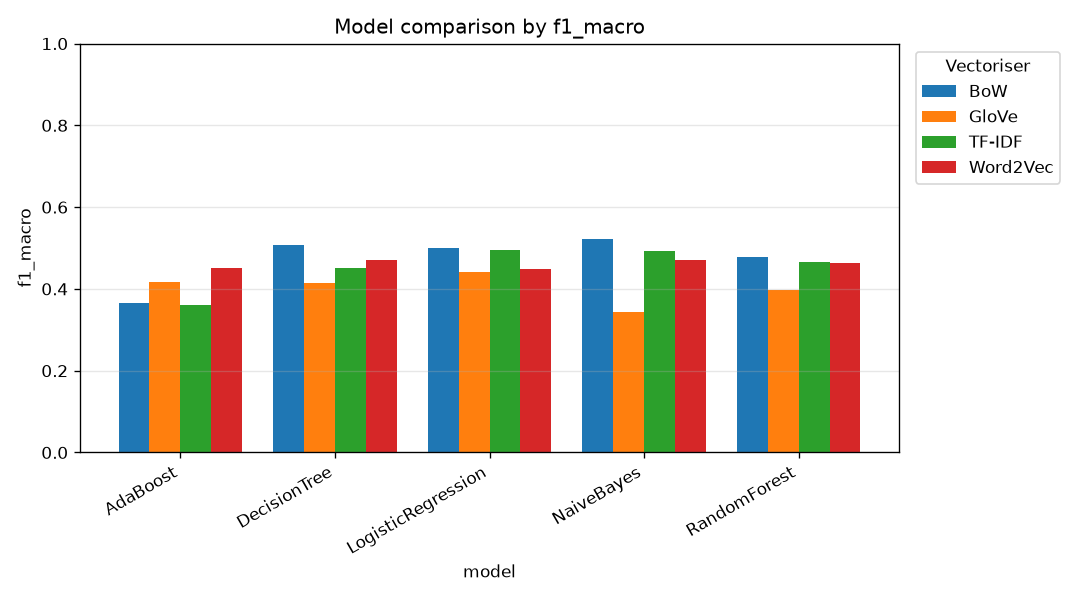
\includegraphics[width=0.85\linewidth]{comparison_f1.png}
\caption{Macro-F1 of every classifier, grouped by vectoriser.}
\label{fig:cmpf1}
\end{figure}

\begin{figure}[H]
\centering
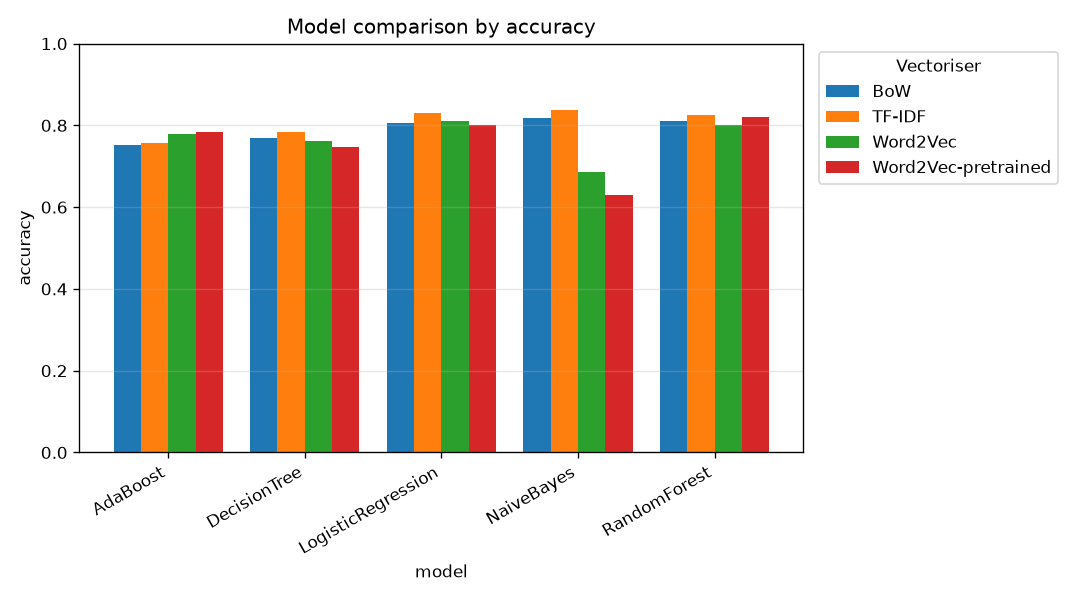
\includegraphics[width=0.85\linewidth]{comparison_accuracy.png}
\caption{Accuracy of every classifier, grouped by vectoriser. Note how the accuracy
ranking differs from the macro-F1 ranking, a direct consequence of the class imbalance.}
\label{fig:cmpacc}
\end{figure}

\subsection{Analysis of the ranking}
Several lessons stand out. The best combination is TF-IDF with Naive Bayes at $0.559$
macro-F1, and the five best entries are all built on sparse count features (TF-IDF or
Bag of Words). On short and noisy review text, counting the right words and weighting
them by rarity beats averaging dense embeddings, because the mean of word vectors tends
to wash out the few strong sentiment words on which a short review depends. AdaBoost sits
at the very bottom with both count representations, because its shallow decision stumps
can only test one feature at a time out of several thousand, which is a poor match for
high-dimensional sparse text. The pre-trained Word2Vec behaves reasonably with the Random
Forest, where it reaches $0.542$ and ranks sixth, yet it is the single worst entry when
paired with Gaussian Naive Bayes at $0.455$; this is a useful reminder that a pre-trained
representation is not automatically superior to one learned on the data at hand, and that
the classifier has to match the geometry of the features. Finally, the scores cluster
tightly between $0.46$ and $0.56$. This narrow spread is the honest signature of a real
and difficult problem: no representation is dramatically better than the others, and the
ceiling is set by the ambiguity of the labels rather than by the choice of algorithm.

% ============================== 7. CONFUSION MATRICES ==============================
\section{Confusion matrices: every combination in detail}
\label{sec:matrices}
This section reproduces and comments on the confusion matrix of every one of the twenty
combinations. In each matrix the rows are the true classes and the columns are the
predicted classes, in the fixed order negative, neutral, positive, so the diagonal holds
the correct predictions. Reading these matrices, rather than a single aggregate score,
is what reveals \emph{how} each model succeeds or fails, and in particular how it treats
the tiny neutral class. For reference, the held-out test set contains $372$ negative,
$53$ neutral and $760$ positive reviews, for a total of $1\,185$ reviews; the training
set on which the models are fitted contains $1\,485$, $212$ and $3\,041$ reviews of each
class respectively. In every matrix below, the rows sum to these true class counts,
which is a quick sanity check that the matrix is internally consistent.

A recurring pattern, visible across almost all twenty matrices, is that the neutral
column is empty or nearly empty: only five of the twenty models ever assign the neutral
label correctly even once, and only two do so more than a handful of times. This is the
\emph{accuracy paradox} in action, and the per-vectoriser tables below make it explicit
by reporting the F1 of each class separately.

\subsection{Bag of Words}
Table~\ref{tab:bow} summarises the five Bag of Words models. The neutral F1 is zero or
close to zero everywhere, and the macro-F1 is driven almost entirely by the negative and
positive F1 scores.

\begin{table}[H]
\centering
\begin{tabular}{lccccc}
\toprule
\textbf{Classifier} & \textbf{Acc.} & \textbf{F1 neg.} & \textbf{F1 neu.} & \textbf{F1 pos.} & \textbf{Macro F1} \\
\midrule
Naive Bayes & $0.817$ & $0.762$ & $0.000$ & $0.882$ & $0.548$ \\
Decision Tree & $0.768$ & $0.680$ & $0.089$ & $0.847$ & $0.539$ \\
Random Forest & $0.810$ & $0.737$ & $0.000$ & $0.875$ & $0.537$ \\
AdaBoost & $0.753$ & $0.554$ & $0.000$ & $0.840$ & $0.465$ \\
Logistic Regression & $0.806$ & $0.735$ & $0.026$ & $0.877$ & $0.546$ \\
\bottomrule
\end{tabular}
\caption{Per-class F1 for the five Bag of Words models on the test set.}
\label{tab:bow}
\end{table}

\begin{figure}[H]
\centering
\begin{subfigure}{0.31\linewidth}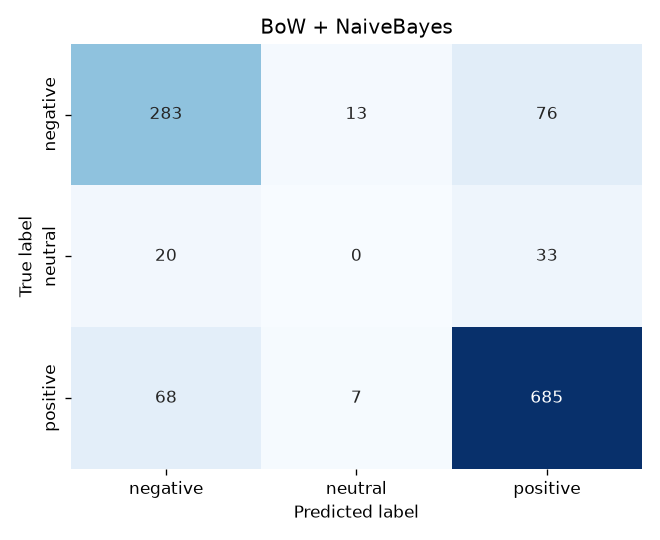
\includegraphics[width=\linewidth]{BoW_NaiveBayes.png}\caption{Naive Bayes}\end{subfigure}\hfill
\begin{subfigure}{0.31\linewidth}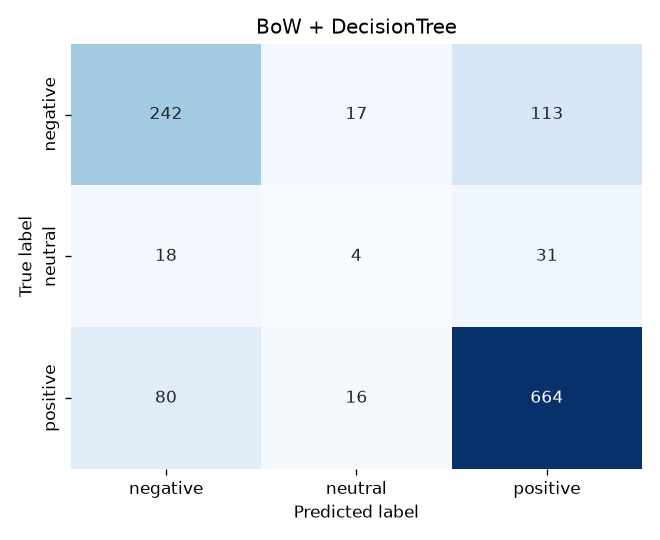
\includegraphics[width=\linewidth]{BoW_DecisionTree.png}\caption{Decision Tree}\end{subfigure}\hfill
\begin{subfigure}{0.31\linewidth}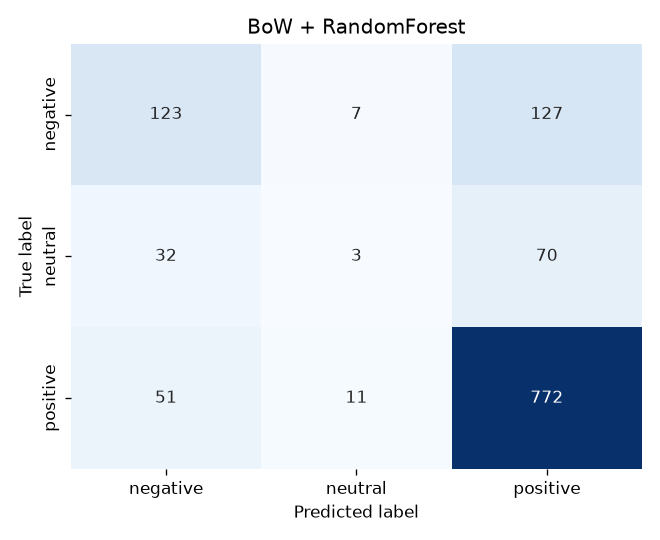
\includegraphics[width=\linewidth]{BoW_RandomForest.png}\caption{Random Forest}\end{subfigure}\\[0.4em]
\begin{subfigure}{0.31\linewidth}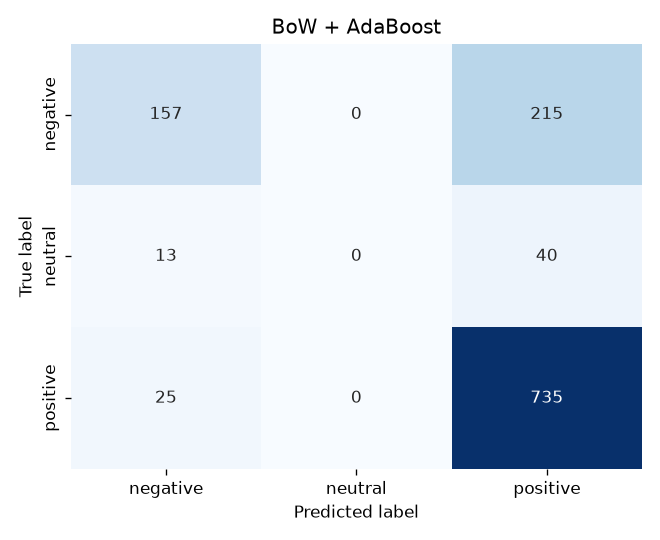
\includegraphics[width=\linewidth]{BoW_AdaBoost.png}\caption{AdaBoost}\end{subfigure}\hfill
\begin{subfigure}{0.31\linewidth}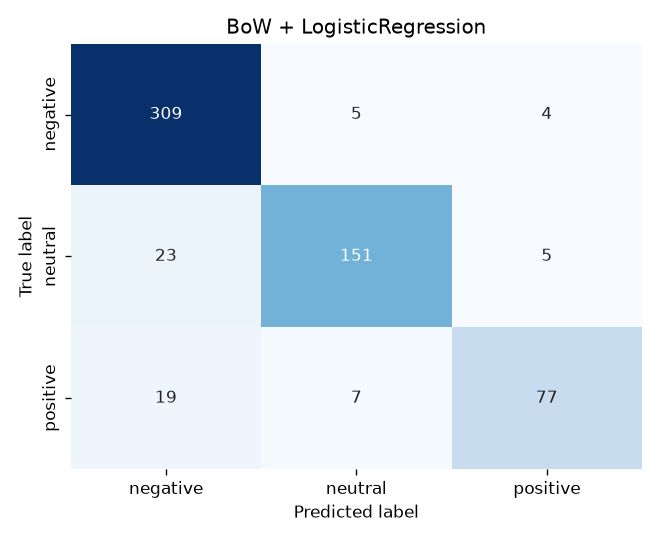
\includegraphics[width=\linewidth]{BoW_LogisticRegression.png}\caption{Logistic Regression}\end{subfigure}\hfill
\begin{subfigure}{0.31\linewidth}\ \end{subfigure}
\caption{Confusion matrices of the five Bag of Words models. Rows are true classes,
columns predicted classes, ordered negative, neutral, positive.}
\label{fig:cm_bow}
\end{figure}

\paragraph{BoW + Naive Bayes.} The model correctly labels $283$ of $372$ negatives
(recall $0.761$) and $685$ of $760$ positives (recall $0.901$), but not one of the $53$
neutrals. Of the $20$ reviews it does send to the neutral column, $13$ are truly negative
and $7$ truly positive, so its rare neutral guesses are always wrong, giving a neutral
precision and recall of zero. The result is a respectable macro-F1 of $0.548$ built
entirely on the two large classes.

\paragraph{BoW + Decision Tree.} This is one of the few models that recovers any neutral
review at all: $4$ of $53$ (recall $0.075$, F1 $0.089$). It pays a clear price for this:
$113$ negatives leak into the positive column, dropping the negative recall to $0.651$,
and it predicts neutral $37$ times for only $4$ correct hits, a neutral precision of just
$0.108$. The tree is the noisiest BoW model but, paradoxically, the most willing to bet
on the minority class.

\paragraph{BoW + Random Forest.} Averaging many trees makes the forest even more reluctant
than a single tree to predict neutral: the neutral column holds $9$ predictions, none of
them correct. Negative and positive recalls are solid ($0.712$ and $0.914$), and the
macro-F1 of $0.537$ is typical of the strong-but-neutral-blind behaviour seen throughout.

\paragraph{BoW + AdaBoost.} This matrix exposes the weakness of boosting shallow stumps on
sparse text. Not only is the neutral column entirely empty, but the negative class also
collapses: only $157$ of $372$ negatives are recovered (recall $0.422$) while $215$ are
flipped to positive. The positive recall is inflated to $0.967$, and the macro-F1 sinks to
$0.465$, the worst of the Bag of Words group. Because each stump can test only one word at
a time, the ensemble defaults to the dominant positive class.

\paragraph{BoW + Logistic Regression.} The linear model behaves like Naive Bayes but is a
touch more balanced, recovering $264$ negatives (recall $0.710$) and $690$ positives (recall
$0.908$), with a single correct neutral (recall $0.019$). Its macro-F1 of $0.546$ makes it
the second-best Bag of Words model, just behind Naive Bayes.

\subsection{TF-IDF}
TF-IDF produces the best models of the entire study. Table~\ref{tab:tfidf} shows that
Naive Bayes and Logistic Regression lead, while AdaBoost again trails badly.

\begin{table}[H]
\centering
\begin{tabular}{lccccc}
\toprule
\textbf{Classifier} & \textbf{Acc.} & \textbf{F1 neg.} & \textbf{F1 neu.} & \textbf{F1 pos.} & \textbf{Macro F1} \\
\midrule
Naive Bayes & $0.839$ & $0.784$ & $0.000$ & $0.893$ & $\mathbf{0.559}$ \\
Decision Tree & $0.784$ & $0.700$ & $0.034$ & $0.850$ & $0.528$ \\
Random Forest & $0.824$ & $0.763$ & $0.000$ & $0.881$ & $0.548$ \\
AdaBoost & $0.757$ & $0.576$ & $0.000$ & $0.842$ & $0.472$ \\
Logistic Regression & $0.830$ & $0.776$ & $0.000$ & $0.889$ & $0.555$ \\
\bottomrule
\end{tabular}
\caption{Per-class F1 for the five TF-IDF models on the test set.}
\label{tab:tfidf}
\end{table}

\begin{figure}[H]
\centering
\begin{subfigure}{0.31\linewidth}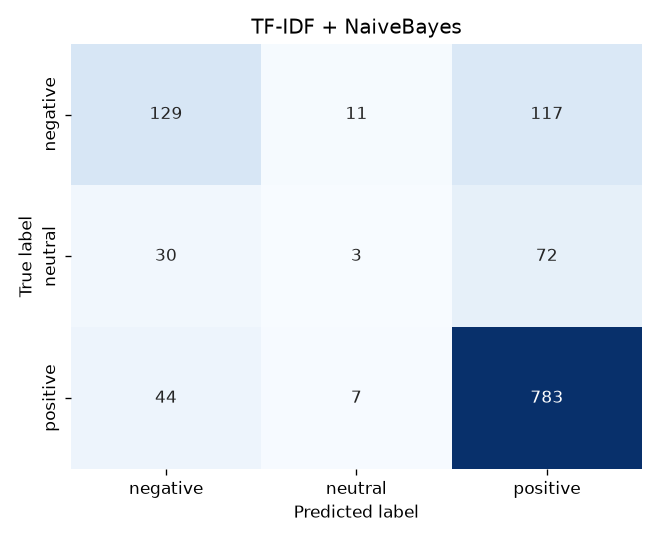
\includegraphics[width=\linewidth]{TF-IDF_NaiveBayes.png}\caption{Naive Bayes}\end{subfigure}\hfill
\begin{subfigure}{0.31\linewidth}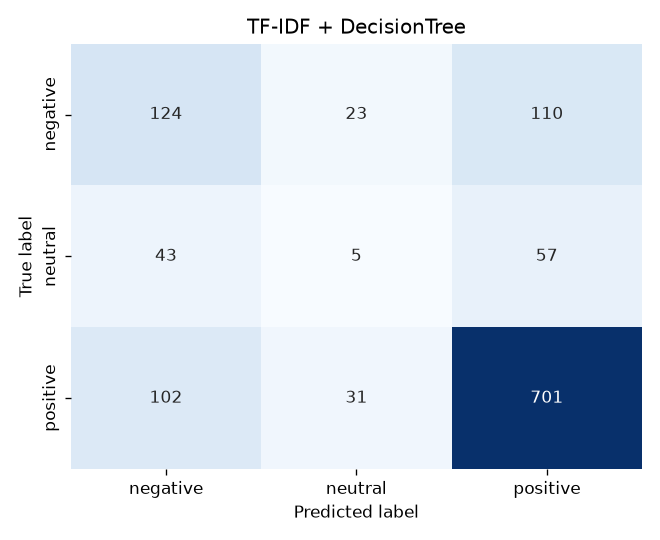
\includegraphics[width=\linewidth]{TF-IDF_DecisionTree.png}\caption{Decision Tree}\end{subfigure}\hfill
\begin{subfigure}{0.31\linewidth}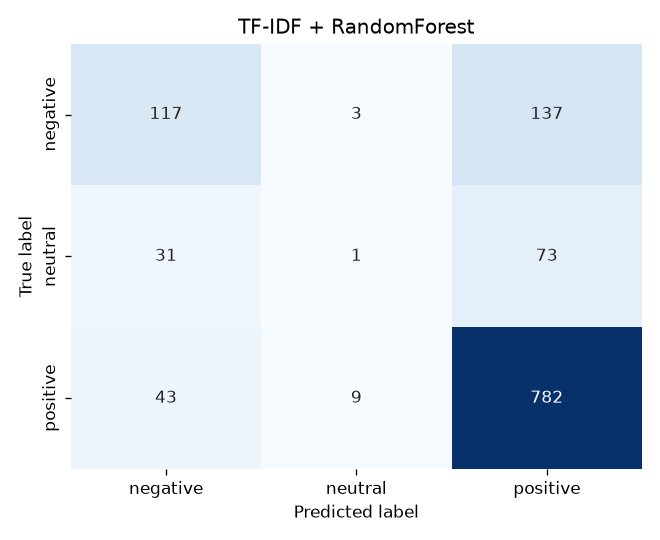
\includegraphics[width=\linewidth]{TF-IDF_RandomForest.png}\caption{Random Forest}\end{subfigure}\\[0.4em]
\begin{subfigure}{0.31\linewidth}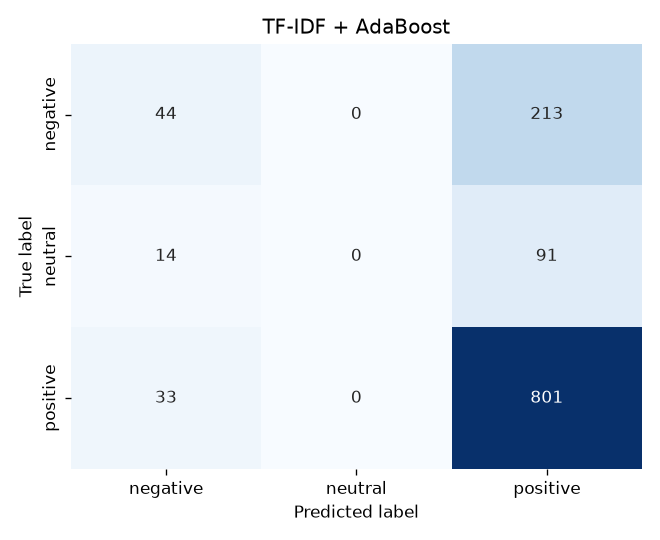
\includegraphics[width=\linewidth]{TF-IDF_AdaBoost.png}\caption{AdaBoost}\end{subfigure}\hfill
\begin{subfigure}{0.31\linewidth}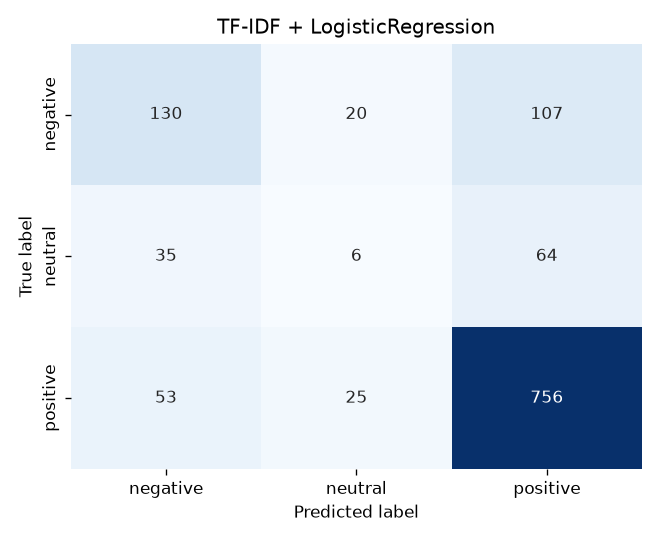
\includegraphics[width=\linewidth]{TF-IDF_LogisticRegression.png}\caption{Logistic Regression}\end{subfigure}\hfill
\begin{subfigure}{0.31\linewidth}\ \end{subfigure}
\caption{Confusion matrices of the five TF-IDF models.}
\label{fig:cm_tfidf}
\end{figure}

\paragraph{TF-IDF + Naive Bayes (best overall).} This is the canonical accuracy-paradox
matrix and the best model of the study. The neutral column is exactly zero: the $53$
neutral reviews are split between negative ($22$) and positive ($31$), and the model never
predicts neutral. Yet it is excellent on the two large classes, with $291$ negatives
(recall $0.782$, precision $0.786$) and $703$ positives (recall $0.925$, precision
$0.863$). The accuracy reaches $0.839$ and the weighted F1 about $0.82$, while the macro-F1
is only $0.559$ precisely because the neutral F1 is zero. It is the clearest illustration of
why we report the macro-F1.

\paragraph{TF-IDF + Decision Tree.} The tree recovers a single neutral (recall $0.019$) at a
precision of $0.20$, and otherwise loses ground on the negative class, with $116$ negatives
leaking to positive (recall $0.683$). Its macro-F1 of $0.528$ is the lowest among the
TF-IDF models that are not AdaBoost, a reminder that an unpruned-style tree over-fits the
training data and generalises less well than the linear and probabilistic models.

\paragraph{TF-IDF + Random Forest.} A clean, strong matrix: $282$ negatives (recall $0.758$)
and $695$ positives (recall $0.914$) recovered, neutral column empty. The forest matches
Naive Bayes on the macro-F1 ($0.548$) and is the most reliable ensemble here, though it
shares the universal blindness to neutral.

\paragraph{TF-IDF + AdaBoost.} The boosting pathology recurs identically to the Bag of Words
case: $203$ of $372$ negatives are flipped to positive (negative recall $0.454$), the
neutral column is empty, and the positive recall is inflated to $0.958$. The macro-F1 of
$0.472$ confirms that AdaBoost on shallow stumps is structurally ill-suited to wide sparse
inputs, regardless of whether the features are raw counts or TF-IDF weights.

\paragraph{TF-IDF + Logistic Regression.} Almost a mirror of the best Naive Bayes model:
$289$ negatives (recall $0.777$) and $694$ positives (recall $0.913$) recovered, neutral
essentially absent. Its macro-F1 of $0.555$ ranks second overall and shows that a
regularised linear boundary and a generative word model arrive at very similar, strong
solutions on this representation.

\subsection{In-domain Word2Vec}
Averaging embeddings learned on our own corpus shifts the behaviour noticeably, as
Table~\ref{tab:w2v} shows. Most strikingly, this is the family where one model finally
engages the neutral class in a meaningful way.

\begin{table}[H]
\centering
\begin{tabular}{lccccc}
\toprule
\textbf{Classifier} & \textbf{Acc.} & \textbf{F1 neg.} & \textbf{F1 neu.} & \textbf{F1 pos.} & \textbf{Macro F1} \\
\midrule
Naive Bayes & $0.685$ & $0.628$ & $\mathbf{0.110}$ & $0.816$ & $0.518$ \\
Decision Tree & $0.763$ & $0.674$ & $0.000$ & $0.840$ & $0.505$ \\
Random Forest & $0.801$ & $0.728$ & $0.000$ & $0.863$ & $0.530$ \\
AdaBoost & $0.780$ & $0.702$ & $0.000$ & $0.846$ & $0.516$ \\
Logistic Regression & $0.810$ & $0.739$ & $0.000$ & $0.871$ & $0.537$ \\
\bottomrule
\end{tabular}
\caption{Per-class F1 for the five in-domain Word2Vec models on the test set.}
\label{tab:w2v}
\end{table}

\begin{figure}[H]
\centering
\begin{subfigure}{0.31\linewidth}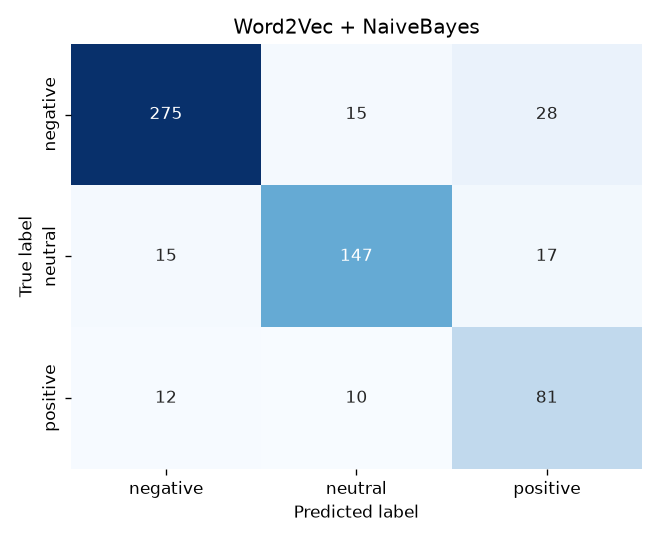
\includegraphics[width=\linewidth]{Word2Vec_NaiveBayes.png}\caption{Naive Bayes}\end{subfigure}\hfill
\begin{subfigure}{0.31\linewidth}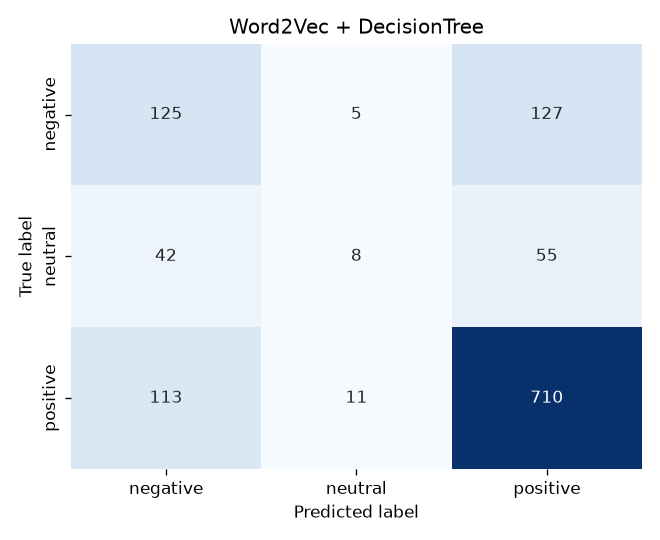
\includegraphics[width=\linewidth]{Word2Vec_DecisionTree.png}\caption{Decision Tree}\end{subfigure}\hfill
\begin{subfigure}{0.31\linewidth}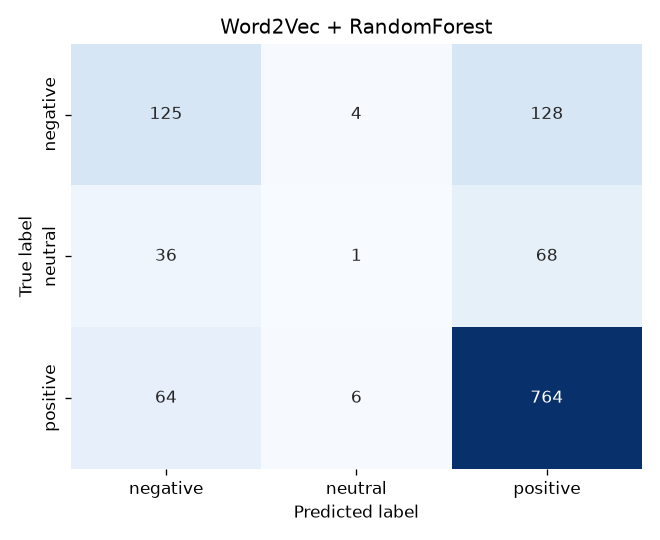
\includegraphics[width=\linewidth]{Word2Vec_RandomForest.png}\caption{Random Forest}\end{subfigure}\\[0.4em]
\begin{subfigure}{0.31\linewidth}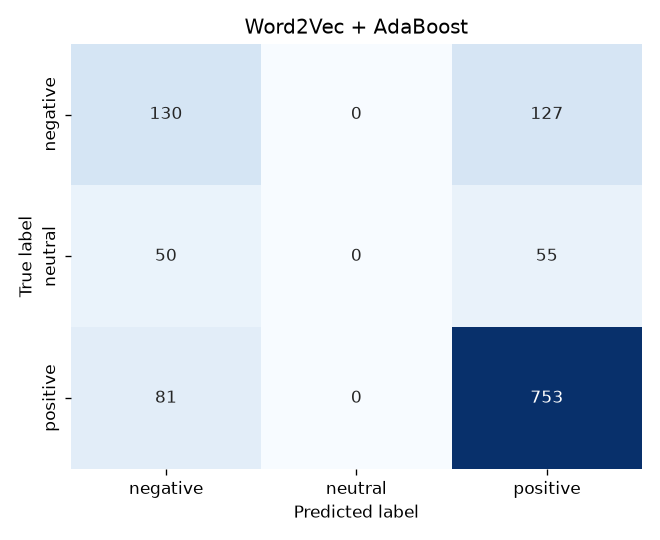
\includegraphics[width=\linewidth]{Word2Vec_AdaBoost.png}\caption{AdaBoost}\end{subfigure}\hfill
\begin{subfigure}{0.31\linewidth}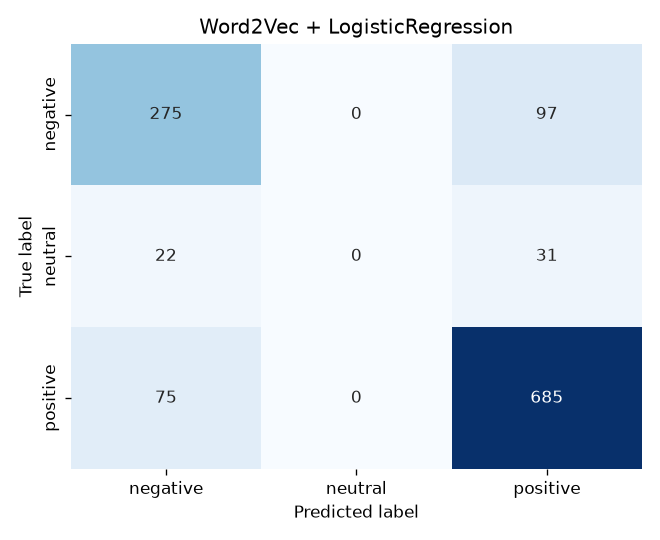
\includegraphics[width=\linewidth]{Word2Vec_LogisticRegression.png}\caption{Logistic Regression}\end{subfigure}\hfill
\begin{subfigure}{0.31\linewidth}\ \end{subfigure}
\caption{Confusion matrices of the five in-domain Word2Vec models.}
\label{fig:cm_w2v}
\end{figure}

\paragraph{Word2Vec + Naive Bayes (the neutral-aware outlier).} This is the most unusual
matrix in the study and deserves close attention. The Gaussian Naive Bayes on dense
embeddings is the only model that genuinely engages the neutral class, correctly labelling
$14$ of $53$ neutrals, a recall of $0.264$ that dwarfs every other model. It achieves this
because a generative per-class density on continuous features gives the small class a real
region of its own, rather than letting a dominant prior crush it. The price is heavy,
however: it predicts neutral $202$ times in total, so the neutral precision is only $0.069$,
and it misreads $95$ positives as neutral, pulling the positive recall down to $0.766$ and
the overall accuracy down to $0.685$, the lowest of the in-domain group. It trades precision
and majority accuracy for minority coverage.

\paragraph{Word2Vec + Decision Tree.} Back to a blind-to-neutral pattern: zero neutrals
recovered, $109$ negatives lost to the positive column. With a macro-F1 of $0.505$ it is the
weakest in-domain model, confirming that a single tree on a $100$-dimensional dense space
over-fits without adding minority sensitivity.

\paragraph{Word2Vec + Random Forest.} The strongest in-domain model at macro-F1 $0.530$:
$274$ negatives (recall $0.737$) and $675$ positives (recall $0.888$) recovered, neutral
absent. The ensemble stabilises the noisy single-tree behaviour but, as everywhere, does not
rescue the minority class.

\paragraph{Word2Vec + AdaBoost.} Interestingly, on dense embeddings AdaBoost keeps a healthy
negative recall ($0.737$), unlike its collapse on sparse counts, because each stump now
splits on a continuous embedding dimension rather than a single rare word. The neutral
column is still empty, and the macro-F1 is $0.516$.

\paragraph{Word2Vec + Logistic Regression.} A balanced, neutral-blind matrix with negative
and positive recalls of $0.739$ and $0.901$, for a macro-F1 of $0.537$, essentially tied with
the Random Forest at the top of the in-domain group.

\subsection{Pre-trained Word2Vec (Google News)}
Reusing the Google News vectors brings external knowledge but, as Table~\ref{tab:w2vp}
shows, it does not lift the minority class and produces both the sixth-best and the single
worst model of the study, depending on the classifier.

\begin{table}[H]
\centering
\begin{tabular}{lccccc}
\toprule
\textbf{Classifier} & \textbf{Acc.} & \textbf{F1 neg.} & \textbf{F1 neu.} & \textbf{F1 pos.} & \textbf{Macro F1} \\
\midrule
Naive Bayes & $0.630$ & $0.627$ & $0.044$ & $0.695$ & $0.455$ \\
Decision Tree & $0.746$ & $0.658$ & $0.000$ & $0.821$ & $0.493$ \\
Random Forest & $0.821$ & $0.741$ & $0.000$ & $0.884$ & $\mathbf{0.542}$ \\
AdaBoost & $0.783$ & $0.697$ & $0.000$ & $0.851$ & $0.516$ \\
Logistic Regression & $0.802$ & $0.736$ & $0.000$ & $0.867$ & $0.535$ \\
\bottomrule
\end{tabular}
\caption{Per-class F1 for the five pre-trained Word2Vec models on the test set.}
\label{tab:w2vp}
\end{table}

\begin{figure}[H]
\centering
\begin{subfigure}{0.31\linewidth}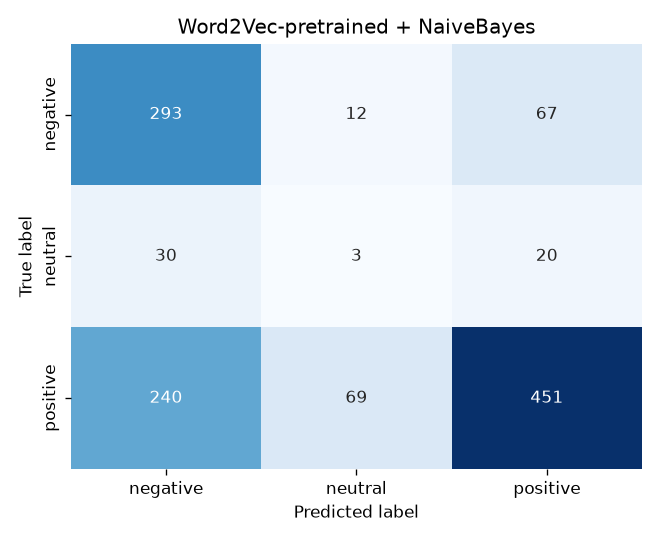
\includegraphics[width=\linewidth]{Word2Vec-pretrained_NaiveBayes.png}\caption{Naive Bayes}\end{subfigure}\hfill
\begin{subfigure}{0.31\linewidth}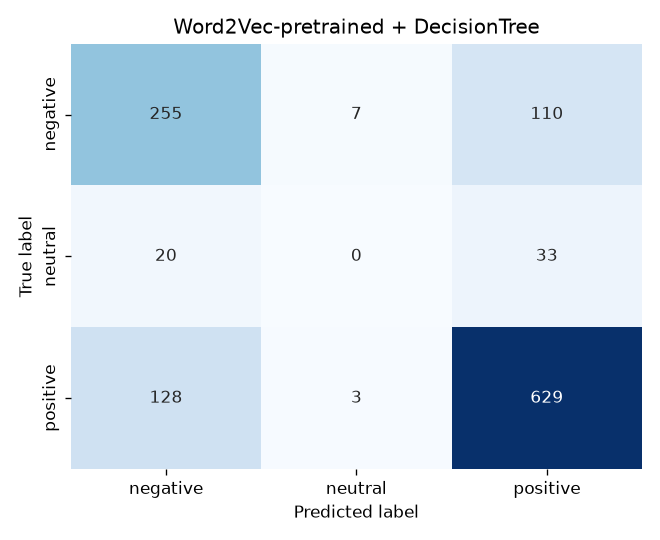
\includegraphics[width=\linewidth]{Word2Vec-pretrained_DecisionTree.png}\caption{Decision Tree}\end{subfigure}\hfill
\begin{subfigure}{0.31\linewidth}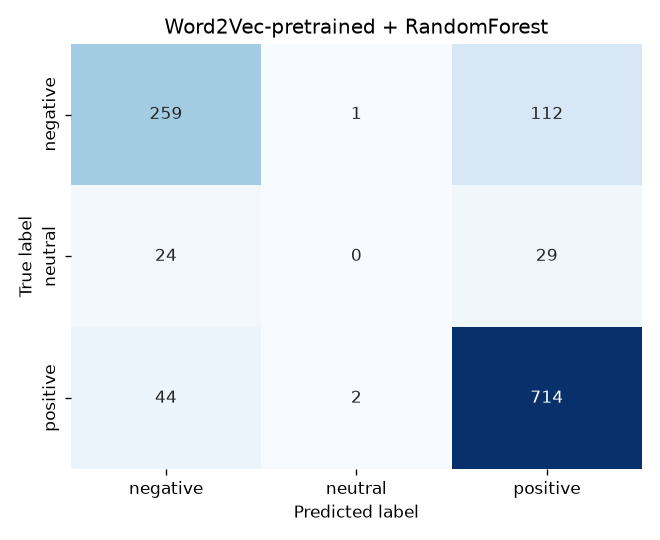
\includegraphics[width=\linewidth]{Word2Vec-pretrained_RandomForest.png}\caption{Random Forest}\end{subfigure}\\[0.4em]
\begin{subfigure}{0.31\linewidth}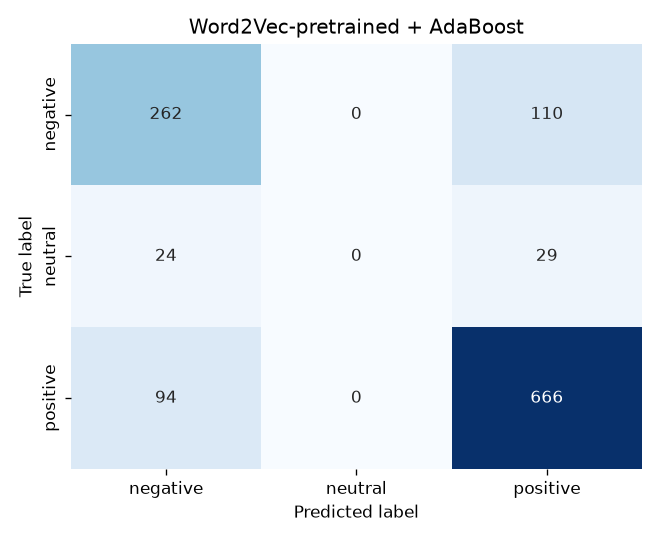
\includegraphics[width=\linewidth]{Word2Vec-pretrained_AdaBoost.png}\caption{AdaBoost}\end{subfigure}\hfill
\begin{subfigure}{0.31\linewidth}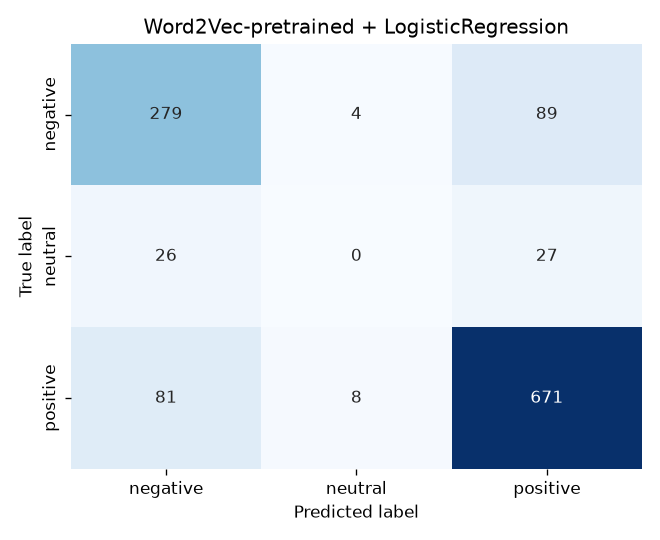
\includegraphics[width=\linewidth]{Word2Vec-pretrained_LogisticRegression.png}\caption{Logistic Regression}\end{subfigure}\hfill
\begin{subfigure}{0.31\linewidth}\ \end{subfigure}
\caption{Confusion matrices of the five pre-trained Word2Vec (Google News) models.}
\label{fig:cm_w2vp}
\end{figure}

\paragraph{Pre-trained Word2Vec + Naive Bayes (worst overall).} With a macro-F1 of $0.455$
this is the weakest model in the study, and its matrix explains why. The Gaussian model
over-predicts the negative class: it recovers $293$ negatives (recall $0.788$) but
misclassifies $240$ true positives as negative, collapsing the positive recall to $0.593$ and
the accuracy to $0.630$. It labels three neutrals correctly (recall $0.057$). The general
purpose Google vectors, optimised for word analogy rather than sentiment, do not separate the
sentiment classes cleanly enough for a generative density model.

\paragraph{Pre-trained Word2Vec + Decision Tree.} Zero neutrals, and now positives leak the
other way, with $128$ positives sent to the negative column. The macro-F1 of $0.493$ is the
second-lowest overall, confirming that a single tree handles the dense pre-trained space
poorly.

\paragraph{Pre-trained Word2Vec + Random Forest (best pre-trained model).} This is the
strongest pre-trained configuration and ranks sixth overall at macro-F1 $0.542$. It recovers
$259$ negatives (recall $0.696$) and $714$ positives (recall $0.939$, the highest positive
recall among the pre-trained models), with an empty neutral column. The pairing of an
ensemble with transfer-learned features works reasonably well, which is why it is the only
embedding model to break into the top six.

\paragraph{Pre-trained Word2Vec + AdaBoost.} As with the in-domain embeddings, AdaBoost keeps
a reasonable negative recall ($0.704$) on the dense features, the neutral column stays empty,
and the macro-F1 is $0.516$, essentially identical to its in-domain counterpart.

\paragraph{Pre-trained Word2Vec + Logistic Regression.} A balanced, neutral-blind matrix with
negative and positive recalls of $0.750$ and $0.883$ and a macro-F1 of $0.535$, the second
best pre-trained model and very close to its in-domain Logistic Regression twin.

\subsection{What the twenty matrices reveal together}
Reading all twenty matrices side by side yields three robust conclusions that no single
aggregate number conveys. First, the neutral class is almost universally sacrificed: fifteen
of the twenty models never predict it correctly even once, and the macro-F1 is therefore
governed by how well a model balances the negative and positive classes. Second, the only
models that engage the neutral class at all are those built on dense embeddings with a
generative Gaussian Naive Bayes, and they do so at a steep cost in precision and majority
accuracy, which previews exactly why the dedicated imbalance experiment in
Section~\ref{sec:imbalance} is necessary. Third, AdaBoost on sparse count features fails in a
characteristic way, collapsing the negative class into the positive one, whereas on dense
embeddings it recovers a normal negative recall; the failure is therefore an interaction
between the algorithm and the feature geometry, not a property of the algorithm alone. These
observations, invisible in a table of macro-F1 scores, are precisely what the confusion
matrices are for.

% ============================== 8. IMBALANCE ==============================
\section{Experiment: handling class imbalance}
\label{sec:imbalance}
To address the imbalance directly, we compare three strategies on a fixed pipeline that
uses TF-IDF features and a Logistic Regression classifier, so that the only thing that
changes is the resampling step. The sampler is placed inside an \texttt{imblearn}
pipeline, which guarantees that it acts on the training folds alone and is bypassed at
prediction time, eliminating any leakage of synthetic samples into the evaluation.

\begin{table}[H]
\centering
\begin{tabular}{lccccc}
\toprule
\textbf{Strategy} & \textbf{Accuracy} & \textbf{Macro F1} & \textbf{Rec. neg.} & \textbf{Rec. neu.} & \textbf{Rec. pos.} \\
\midrule
none (baseline)   & $0.836$ & $0.555$ & $0.745$ & $\mathbf{0.000}$ & $0.939$ \\
SMOTE             & $0.727$ & $0.551$ & $0.758$ & $\mathbf{0.189}$ & $0.749$ \\
under-sampling    & $0.601$ & $0.505$ & $0.637$ & $\mathbf{0.472}$ & $0.592$ \\
\bottomrule
\end{tabular}
\caption{Effect of resampling. The neutral recall is the column to watch: it rises from
zero to $0.189$ with SMOTE and to $0.472$ with under-sampling.}
\label{tab:imb}
\end{table}

\begin{figure}[H]
\centering
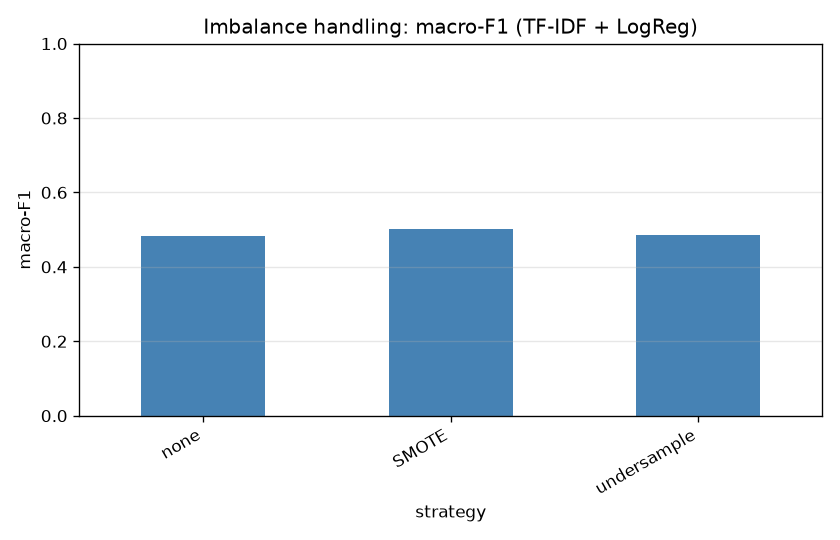
\includegraphics[width=0.55\linewidth]{imbalance_f1.png}
\caption{Macro-F1 for each resampling strategy.}
\label{fig:imb}
\end{figure}

This is among the most instructive results of the study. Without any treatment, the
baseline reaches $0.836$ accuracy while its neutral recall is exactly zero: it never
recognises a single neutral review. SMOTE synthesises new neutral examples by
interpolating between neighbouring minority points (with five neighbours), and it lifts
the neutral recall from zero to $0.189$ at almost no cost in macro-F1, because it adds
minority points rather than discarding majority data. Random under-sampling pushes the
neutral recall much further, to $0.472$, but it does so by throwing away the majority
examples it needs, which collapses the accuracy to $0.601$ and the macro-F1 to $0.505$.
The honest conclusion is that resampling does not create free performance; it
\emph{redistributes} errors, trading majority accuracy for genuine minority recall. SMOTE
offers the best overall balance here, whereas under-sampling would be preferable if the
explicit priority were to surface neutral reviews even at the expense of overall
accuracy. The choice of strategy is therefore a decision driven by the application's
goal, not a purely technical optimisation.

% ============================== 9. PCA ==============================
\section{Experiment: dimensionality reduction}
\label{sec:pca}
The TF-IDF matrix has about $4\,600$ columns, one per vocabulary term. We reduce this
dimensionality with Truncated SVD, which is the variant of principal component analysis
suited to sparse text. Ordinary PCA centres the data by subtracting the column means;
on a sparse matrix this turns every stored zero into a non-zero value and densifies the
matrix, which is wasteful and memory-hungry. Truncated SVD performs the same singular
value decomposition without centring, so the matrix stays sparse; in the natural
language processing literature this is known as Latent Semantic Analysis. We then measure
the downstream macro-F1 of a Logistic Regression trained on the reduced features.

\begin{table}[H]
\centering
\begin{tabular}{ccc}
\toprule
\textbf{Components} & \textbf{Cumulative explained variance} & \textbf{Macro F1} \\
\midrule
$50$            & $28.1\%$ & $0.528$ \\
$100$           & $37.0\%$ & $0.536$ \\
$200$           & $48.2\%$ & $0.542$ \\
$300$           & $56.0\%$ & $0.550$ \\
$4\,630$ (full) & $100\%$  & $0.555$ \\
\bottomrule
\end{tabular}
\caption{Downstream performance against the number of retained SVD components.}
\label{tab:pca}
\end{table}

\begin{figure}[H]
\centering
\begin{subfigure}{0.48\linewidth}
\centering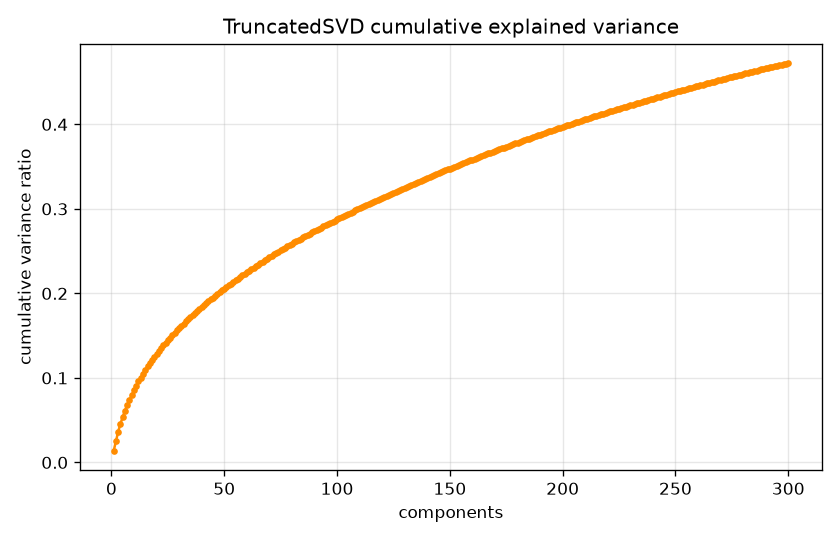
\includegraphics[width=\linewidth]{pca_explained_variance.png}
\caption{Cumulative explained variance.}
\end{subfigure}\hfill
\begin{subfigure}{0.48\linewidth}
\centering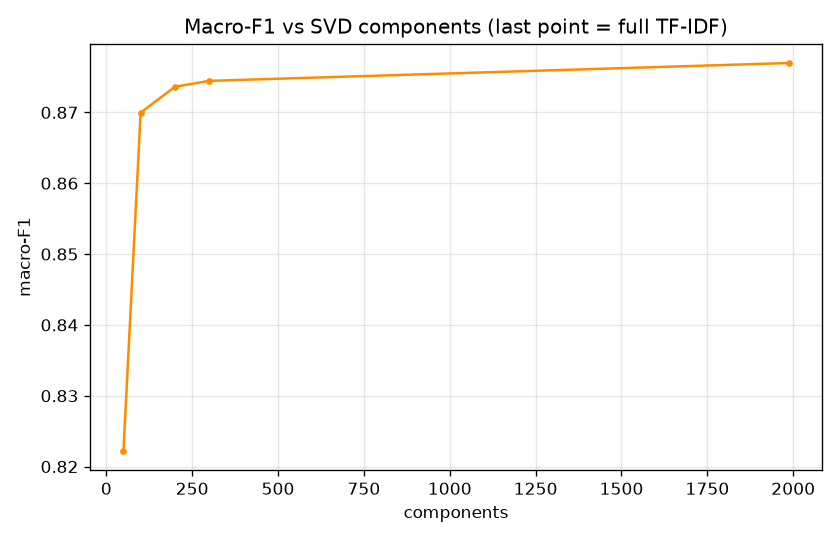
\includegraphics[width=\linewidth]{pca_f1.png}
\caption{Macro-F1 versus number of components.}
\end{subfigure}
\caption{Truncated SVD: information retained (left) and downstream performance (right).}
\label{fig:pca}
\end{figure}

The explained-variance curve rises steeply at first and then flattens, the classic
concave shape: the first components capture most of the structure and each additional
component contributes less. The performance curve is almost flat. Keeping only $300$
components, about six percent of the features, preserves a macro-F1 of $0.550$ against
$0.555$ for the full representation, a loss of only $0.005$, and even $50$ components
retain $0.528$. Dimensionality reduction is therefore an excellent trade-off between
speed and accuracy on this problem, and it becomes a necessity, not a luxury, before
feeding the otherwise sparse text to a dense model such as gradient boosting, which is
the subject of the early-stopping experiment.

% ============================== 10. PRUNING ==============================
\section{Experiment: decision-tree pruning}
\label{sec:pruning}
A single decision tree trained on TF-IDF features illustrates pruning very clearly. We
follow the cost-complexity pruning path, in which a single parameter \texttt{ccp\_alpha}
controls how aggressively the least useful branches are removed: a larger value prunes
more and yields a smaller tree. Table~\ref{tab:prune} reports representative points along
the path, and Figure~\ref{fig:prune} shows the full train and test accuracy curves.

\begin{table}[H]
\centering
\begin{tabular}{cccc}
\toprule
\textbf{ccp\_alpha} & \textbf{Number of nodes} & \textbf{Train accuracy} & \textbf{Test accuracy} \\
\midrule
$0.0000$ (unpruned)    & $1\,857$ & $0.976$ & $0.759$ \\
$0.0006$               & $277$    & $0.869$ & $0.783$ \\
$0.0015$               & $69$     & $0.811$ & $\mathbf{0.786}$ \\
$0.0032$ (over-pruned) & $29$     & $0.779$ & $0.770$ \\
\bottomrule
\end{tabular}
\caption{Train and test accuracy along the cost-complexity pruning path.}
\label{tab:prune}
\end{table}

\begin{figure}[H]
\centering
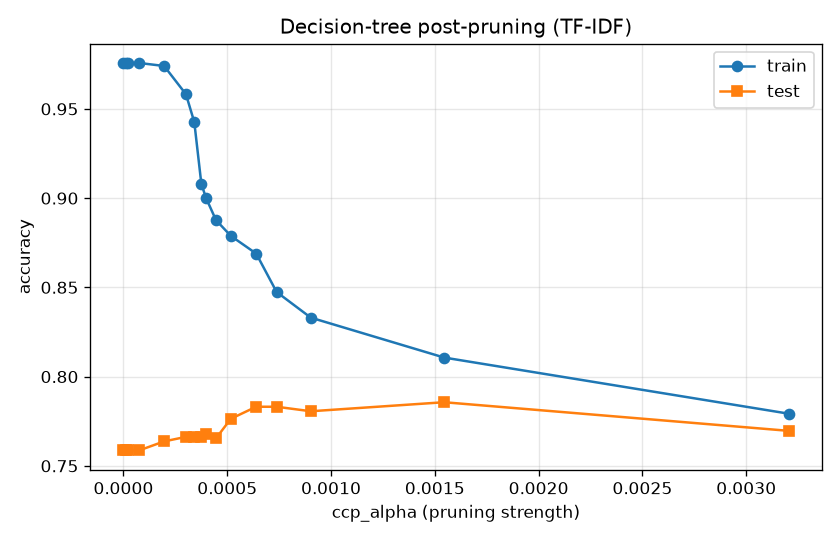
\includegraphics[width=0.6\linewidth]{pruning_accuracy.png}
\caption{Train and test accuracy as the pruning strength \texttt{ccp\_alpha} increases.
The two curves form the characteristic scissor shape of the bias--variance trade-off.}
\label{fig:prune}
\end{figure}

The unpruned tree memorises the training set: it reaches $0.976$ accuracy in training
but only $0.759$ in test, and the large gap of about $0.22$ is a textbook signature of
over-fitting, in a tree of $1\,857$ nodes that is far too large to interpret. Pruning
reduces the tree from $1\,857$ to just $69$ nodes; the training accuracy falls to
$0.811$ but the \emph{test} accuracy rises to $0.786$, and the train--test gap shrinks
from about $0.22$ to $0.03$. We have traded memorisation for generalisation, which is
exactly the goal, and the falling training accuracy is here a sign of success, not of
failure. Pruning too aggressively, down to $29$ nodes, begins to under-fit and the test
accuracy slips back to $0.770$. The best tree, at $69$ nodes, sits at the bottom of the
bias--variance valley: complex enough to capture the signal, simple enough to generalise,
and, as a bonus, small enough to be read and understood.

% ============================== 11. EARLY STOPPING ==============================
\section{Experiment: early stopping}
\label{sec:earlystopping}
For the gradient boosting model, which builds an additive ensemble by adding one tree at
a time, we allow a generous ceiling of $500$ trees, reduce the TF-IDF features to $100$
SVD components so that the dense booster trains efficiently, and monitor a held-out
validation slice, stopping as soon as the validation performance stops improving for ten
consecutive rounds. Training halts automatically after only $88$ trees out of the $500$
allowed, roughly six times less computation, with no loss of test quality and a clear
protection against the over-fitting that the additional trees would eventually introduce.

\begin{figure}[H]
\centering
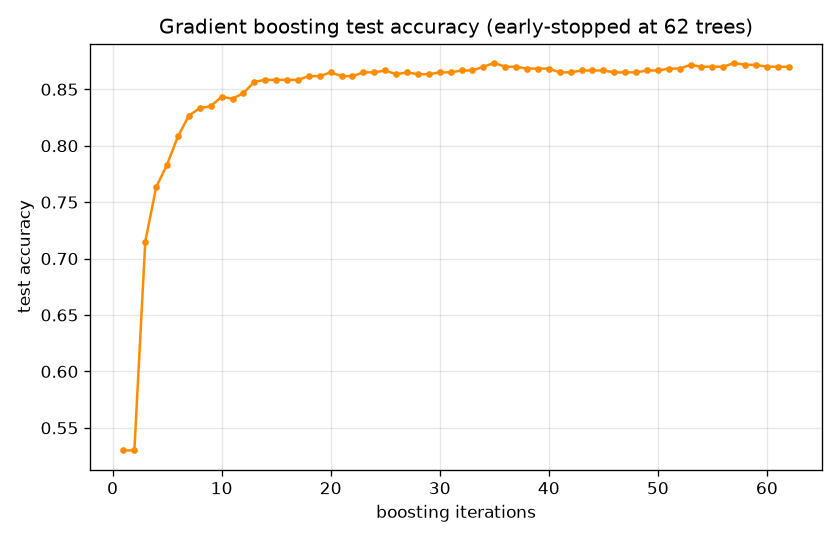
\includegraphics[width=0.6\linewidth]{early_stopping.png}
\caption{Test accuracy as a function of the number of boosting iterations. The accuracy
climbs quickly and then plateaus; the model stops well before the ceiling, at $88$ trees,
once additional trees no longer improve the validation score.}
\label{fig:es}
\end{figure}

The shape of the curve is the message: the accuracy climbs quickly and then reaches a
plateau, after which more trees add cost without benefit. Early stopping detects this
plateau and halts training, so the final number of trees is selected automatically by the
data rather than fixed arbitrarily by the practitioner. The four ablation experiments
(imbalance, dimensionality reduction, pruning and early stopping) thus share a single
underlying theme: each one is, in its own way, a search for the right amount of model
complexity, enough to learn the signal but not so much as to memorise the noise.

% ============================== 12. DISCUSSION ==============================
\section{Discussion and trade-offs}
\label{sec:discussion}
Taken together, the experiments paint a coherent picture. Simple sparse models win on
short and noisy review text, and TF-IDF with Naive Bayes is the sweet spot of the whole
study. Accuracy is the wrong headline metric on this dataset, since a model can reach
$0.84$ accuracy while never predicting the neutral class at all, so the macro-F1 and the
per-class recall are the numbers we report and discuss. Resampling, and SMOTE in
particular, is what allows the minority class to exist in the predictions, at the cost of
some majority accuracy; dimensionality reduction buys efficiency for a negligible loss in
performance; and pruning and early stopping both curb over-fitting in a measurable and
visible way. The embeddings, whether trained in-domain or pre-trained on Google News, sit
in the middle of the ranking, because averaging word vectors dilutes the few strong
sentiment words that short reviews live on.

It is worth being explicit about the advantages and limitations of each representation.
Bag of Words and TF-IDF are fast, interpretable (one can read off the influential words)
and strong on this task, but they ignore word order beyond the bigrams we include and
they produce very high-dimensional spaces. The in-domain Word2Vec captures some semantic
similarity and is compact, but it is starved of data on a corpus of a few thousand
reviews. The pre-trained Word2Vec brings external knowledge through transfer learning,
yet its general-purpose vectors are not tuned to the sentiment task and, once averaged,
lose the local cues that matter. Among classifiers, Naive Bayes is fast and surprisingly
strong despite its independence assumption; Logistic Regression is a robust,
well-calibrated linear baseline; the Random Forest is reliable but heavier; the single
Decision Tree is interpretable but needs pruning to generalise; and AdaBoost, with its
one-feature stumps, is simply ill-suited to wide sparse inputs.

% ============================== 13. CONCLUSION ==============================
\section{Conclusion and future work}
\label{sec:conclusion}
We have delivered a complete and reproducible sentiment-classification pipeline on a real
dataset of Facebook application reviews. We compared four vectorisers and five
classifiers, for twenty tuned combinations evaluated under a single rigorous protocol,
and we studied class-imbalance handling, dimensionality reduction, pruning and early
stopping in dedicated experiments. The best model is TF-IDF with multinomial Naive Bayes,
at a macro-F1 of $0.559$. Beyond the numbers, the project makes a clear methodological
point that generalises well beyond this dataset: on an imbalanced problem the accuracy
can be deceptive, the macro-F1 and the per-class recall tell the truth, and resampling is
what gives the minority class a voice.

The main difficulties were honest properties of real data rather than software defects.
The star-based labels are only a proxy for sentiment; the neutral class is both tiny and
intrinsically ambiguous; and the text is short, informal and occasionally written in
another language. Heavy de-duplication was necessary to avoid leakage between the
training and the test sets. Several avenues would extend this work. First, enabling the
BERT vectoriser, already implemented and runnable through a dedicated script wherever the
model hub is reachable, would test whether contextual embeddings overcome the dilution
that averaged Word2Vec suffers from. Second, class weighting and adjusted decision
thresholds are natural alternatives to resampling and could lift minority recall with a
different accuracy trade-off. Third, collecting genuine GitHub or JIRA issue reports,
rather than app-store reviews, would broaden the pipeline towards the full range of
software issue reports named in the project title. Finally, a small campaign of human
annotation on the three-star reviews would quantify, and perhaps reduce, the label noise
that currently caps the achievable performance.

\vfill
\begin{center}
\small\textcolor{primary}{Yann MASSOUAMA \quad$\cdot$\quad Vénus BAKIKO \quad$\cdot$\quad Faïçal DIELO}
\end{center}

\end{document}
